\chapter{Hardware, Memory, And Backends}

A training project becomes more valuable when it separates the model concept from the
implementation backend. The same GPT architecture can be implemented in PyTorch for
teaching, Candle for Rust-native systems work, and C/CUDA for low-level performance
study. The hardware chapter explains what those backends are actually asking the machine
to do.

The central lesson is:

\begin{quote}
Hardware does not change the mathematics of GPT, but it strongly changes which model
sizes, batch sizes, dtypes, kernels, and file formats are practical.
\end{quote}

\section{Learning Objectives}

By the end of this chapter, students should be able to:

\begin{itemize}
  \item estimate memory used by parameters, gradients, optimizer state, activations, and
  KV cache;
  \item explain why a checkpoint file is smaller than the memory needed for training;
  \item compute effective batch size in gradient accumulation and DDP;
  \item distinguish PyTorch, Candle, llm.c, and GGUF runtime roles;
  \item design a fair backend comparison using loss, throughput, memory, and samples;
  \item decide which backend is appropriate for learning, Rust integration, kernel study,
  or local inference.
\end{itemize}

\section{What Hardware Does In LLM Training}

Training a GPT model is a repeated movement of tensors:

\[
\text{load token batch}
\rightarrow
\text{forward pass}
\rightarrow
\text{loss}
\rightarrow
\text{backward pass}
\rightarrow
\text{optimizer update}.
\]

Hardware determines how fast and how large this cycle can be.

\begin{figure}[htbp]
\centering
\resizebox{\textwidth}{!}{%
\begin{tikzpicture}[
  box/.style={draw, rounded corners, minimum width=2.55cm, minimum height=0.75cm, align=center},
  arrow/.style={-{Latex[length=3mm]}, thick}
]
\node[box, fill=blue!6] (disk) at (0,0) {disk\\token shards};
\node[box, fill=yellow!18] (cpu) at (3.0,0) {CPU\\batching};
\node[box, fill=orange!14] (gpu) at (6.0,0) {GPU\\forward/backward};
\node[box, fill=green!10] (opt) at (9.0,0) {optimizer\\state update};
\node[box, fill=red!8] (ckpt) at (12.0,0) {checkpoint\\write};
\draw[arrow] (disk) -- (cpu);
\draw[arrow] (cpu) -- (gpu);
\draw[arrow] (gpu) -- (opt);
\draw[arrow] (opt) -- (ckpt);
\draw[arrow] (opt.south) .. controls +(0,-1.2) and +(0,-1.2) .. (cpu.south);
\end{tikzpicture}}
\caption{A training step is a hardware pipeline, not only a Python loop.}
\end{figure}

The GPU performs most tensor arithmetic. The CPU prepares batches, launches work, handles
some logging, and writes files. Disk supplies token shards and stores checkpoints. The
slowest part of this pipeline can dominate training time.

\section{GPU Memory Categories}

Training memory includes several categories:

\begin{itemize}
  \item \textbf{parameters}: learned model weights;
  \item \textbf{gradients}: derivatives for those weights;
  \item \textbf{optimizer state}: AdamW moment estimates \(m\) and \(v\);
  \item \textbf{master weights}: sometimes kept in FP32 during mixed precision training;
  \item \textbf{activations}: intermediate tensors saved for the backward pass;
  \item \textbf{temporary workspaces}: buffers used by kernels and libraries;
  \item \textbf{input and target batches}: token IDs and labels;
  \item \textbf{communication buffers}: used by distributed training.
\end{itemize}

This is why a checkpoint file does not directly tell you required GPU memory. A checkpoint
may store model weights and optimizer state, but training also needs activations and
temporary buffers.

\section{Parameter Memory}

Suppose a model has \(P\) parameters. The raw parameter memory is:

\[
\text{parameter bytes} = P \times \text{bytes per parameter}.
\]

Common dtypes:

\begin{longtable}{p{0.18\textwidth}p{0.18\textwidth}p{0.46\textwidth}}
\toprule
\term{dtype} & \term{bytes/value} & \term{Common role} \\
\midrule
FP32 & 4 & stable training, optimizer state, master weights \\
FP16 & 2 & mixed precision training/inference on supported GPUs \\
BF16 & 2 & mixed precision with wider exponent, hardware dependent \\
INT8 & 1 & quantized inference or specialized training paths \\
4-bit & 0.5 & quantized inference formats such as many GGUF variants \\
\bottomrule
\end{longtable}

\section{AdamW Memory}

AdamW stores two moment estimates for each parameter:

\[
m_t,\quad v_t.
\]

If each is FP32, optimizer state alone costs:

\[
2 \times P \times 4\ \text{bytes} = 8P\ \text{bytes}.
\]

A rough mixed precision AdamW training memory estimate per parameter can be:

\[
\text{param} + \text{grad} + \text{master param} + m + v.
\]

Depending on implementation details, this may be roughly:

\[
2P + 2P\text{ or }4P + 4P + 4P + 4P
\]

bytes before activations. The exact number depends on the backend, dtype policy, fused
optimizer, and whether FP32 master weights are kept.

\section{Activation Memory}

Activations often dominate training memory. During the forward pass, the backend saves
intermediate tensors so backward pass can compute gradients. A rough shape-based way to
think about activation memory is:

\[
\text{activation scale} \propto B \times T \times C \times L.
\]

Here:

\begin{itemize}
  \item \(B\) is microbatch size;
  \item \(T\) is context length;
  \item \(C\) is embedding dimension;
  \item \(L\) is number of Transformer blocks.
\end{itemize}

The real multiplier is larger because attention, MLP, normalization, dropout, residuals,
and temporary tensors all create additional storage.

\begin{figure}[htbp]
\centering
\resizebox{\textwidth}{!}{%
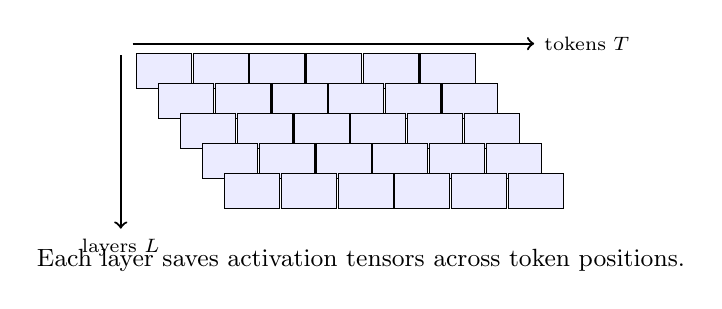
\begin{tikzpicture}[
  cell/.style={draw, minimum width=0.7cm, minimum height=0.45cm, fill=blue!8},
  lab/.style={font=\small, align=center}
]
\foreach \l in {0,...,4} {
  \foreach \t in {0,...,5} {
    \node[cell] at (\t*0.72+\l*0.28,-\l*0.38) {};
  }
}
\draw[->, thick] (-0.4,0.35) -- (4.7,0.35) node[right] {\scriptsize tokens \(T\)};
\draw[->, thick] (-0.55,0.2) -- (-0.55,-2.0) node[below] {\scriptsize layers \(L\)};
\node[lab] at (2.5,-2.4) {Each layer saves activation tensors across token positions.};
\end{tikzpicture}}
\caption{Activation memory grows with sequence length, hidden dimension, batch size, and layer count.}
\end{figure}

\section{Why Gradient Accumulation Helps}

Gradient accumulation lets a small GPU simulate a larger effective batch. If the GPU can
only fit a microbatch of \(B_{\text{micro}}\), we can run several microbatches, accumulate
gradients, then update once:

\[
B_{\text{effective}} =
B_{\text{micro}} \times
\text{gradient accumulation steps} \times
\text{world size}.
\]

Gradient accumulation usually does \emph{not} multiply peak activation memory by the
accumulation count, because microbatches are processed one at a time. It does increase
wall-clock time per optimizer update.

\section{Distributed Data Parallel Training}

Distributed Data Parallel, or DDP, creates one model replica per worker. Each worker
receives a different microbatch. After backward pass, gradients are averaged across
workers, usually by an all-reduce operation.

\begin{figure}[htbp]
\centering
\resizebox{\textwidth}{!}{%
\begin{tikzpicture}[
  box/.style={draw, rounded corners, minimum width=2.5cm, minimum height=0.75cm, align=center},
  arrow/.style={-{Latex[length=3mm]}, thick}
]
\node[box, fill=blue!6] (gpu0) at (0,0) {GPU 0\\model copy};
\node[box, fill=blue!6] (gpu1) at (4,0) {GPU 1\\model copy};
\node[box, fill=yellow!18] (b0) at (0,1.2) {microbatch A};
\node[box, fill=yellow!18] (b1) at (4,1.2) {microbatch B};
\node[box, fill=green!10] (sync) at (2,-1.25) {gradient\\all-reduce};
\draw[arrow] (b0) -- (gpu0);
\draw[arrow] (b1) -- (gpu1);
\draw[arrow] (gpu0) -- (sync);
\draw[arrow] (gpu1) -- (sync);
\draw[arrow] (sync) -- (gpu0);
\draw[arrow] (sync) -- (gpu1);
\end{tikzpicture}}
\caption{DDP synchronizes gradients so each model replica applies the same optimizer update.}
\end{figure}

DDP improves throughput only when the extra parallel compute is worth the communication
cost. On small consumer GPUs, tiny microbatches and slow interconnects can limit speedup.

\section{Case Study: GPT21 Parameter And Memory Estimate}

The GPT21 WikiText-103 run used:

\[
V=32000,\quad T=512,\quad L=6,\quad H=6,\quad C=384.
\]

The token embedding table alone has:

\[
V \times C = 32000 \times 384 = 12{,}288{,}000
\]

parameters. The position embedding table has:

\[
T \times C = 512 \times 384 = 196{,}608
\]

parameters.

Each Transformer block has approximate major weight matrices:

\begin{longtable}{p{0.36\textwidth}p{0.26\textwidth}p{0.22\textwidth}}
\toprule
\term{Component} & \term{Approximate shape} & \term{Parameters} \\
\midrule
QKV projection & \(C \times 3C\) & \(384 \times 1152\) \\
Attention output projection & \(C \times C\) & \(384 \times 384\) \\
MLP up projection & \(C \times 4C\) & \(384 \times 1536\) \\
MLP down projection & \(4C \times C\) & \(1536 \times 384\) \\
LayerNorm parameters & several vectors of length \(C\) & small compared with matrices \\
\bottomrule
\end{longtable}

A rough model-size estimate is about 23 million parameters if the token embedding and
output head are tied, or about 35 million if they are untied. This explains why a
checkpoint around 265 MiB can be plausible when it includes more than FP16 inference
weights, such as optimizer state or FP32 tensors.

\section{Case Study: wish01 PyTorch Baseline}

\term{REPORTED historical case study, not reproduced by this repository.}
The original manuscript describes a \texttt{wish01} GPT21 run with the following
configuration. Its raw logs, hardware manifest and code revision are not bundled
here, so the figures below must not be advertised as a verified benchmark:

\begin{itemize}
  \item model shape \(V=32000,T=512,L=6,H=6,C=384\);
  \item mixed precision \texttt{float16};
  \item \texttt{micro\_batch\_size = 1};
  \item \texttt{gradient\_accumulation\_steps = 32};
  \item 10000 optimizer steps;
  \item checkpoint every 500 steps.
\end{itemize}

If the run uses two workers, the effective batch is:

\[
B_{\text{effective}} = 1 \times 2 \times 32 = 64
\]

sequences per optimizer step, or:

\[
64 \times 512 = 32768
\]

token positions per optimizer step. Across 10000 optimizer steps:

\[
32768 \times 10000 = 327{,}680{,}000
\]

token positions are processed. With an observed wall time of about 20 hours and 37
minutes, the approximate throughput is:

\[
\frac{327{,}680{,}000\ \text{tokens}}{74231\ \text{seconds}}
\approx 4414\ \text{tokens/second}.
\]

This is a \term{DERIVED} ratio of reported totals, conditional on two workers
actually processing the stated batch. It is not a new measurement or an
audited baseline. Reproduction requires the missing run manifest and logs.

\section{Memory Levers}

If training runs out of memory, common levers are:

\begin{longtable}{p{0.28\textwidth}p{0.48\textwidth}p{0.12\textwidth}}
\toprule
\term{Lever} & \term{Effect} & \term{Tradeoff} \\
\midrule
Reduce microbatch size & lowers activation memory & noisier step unless accumulating \\
Reduce block size \(T\) & lowers activation and attention memory & shorter context \\
Reduce layer count \(L\) & lowers parameters and activations & smaller model \\
Reduce embedding size \(C\) & strongly lowers matrix sizes & smaller model \\
Use gradient accumulation & increases effective batch without larger microbatch & slower optimizer steps \\
Use mixed precision & lowers tensor memory and improves speed on supported hardware & numerical care \\
Activation checkpointing & saves fewer activations, recomputes during backward & more compute \\
Use a fused optimizer & reduces overhead and temporary buffers & backend-dependent \\
Quantize for inference & reduces inference memory & not usually for full training resume \\
\bottomrule
\end{longtable}

\section{Backend Execution Models}

The same model contract appears differently in each backend.

\subsection{PyTorch}

PyTorch is the best first backend because it provides:

\begin{itemize}
  \item dynamic computation graphs;
  \item automatic differentiation;
  \item mature DDP;
  \item easy tensor inspection;
  \item rich debugging tools.
\end{itemize}

The price is that much of the memory layout and kernel scheduling is hidden. That is good
for learning the model, but less direct for learning systems internals.

\subsection{Candle}

Candle brings the model into Rust. Its value is not merely speed; it changes the
engineering boundary:

\begin{itemize}
  \item configs become typed Rust structures;
  \item errors become explicit \texttt{Result<T>} values;
  \item checkpoints can align naturally with safetensors;
  \item inference can live closer to Rust services or desktop applications.
\end{itemize}

Candle should use the same token files, model config, and evaluation prompts as PyTorch.
Otherwise, the comparison is not meaningful.

\subsection{llm.c And C/CUDA}

llm.c-style code makes memory and kernels visible:

\begin{itemize}
  \item parameters can be flat buffers;
  \item activation memory is explicitly allocated;
  \item backward kernels are explicit;
  \item optimizer state is manually organized;
  \item throughput and memory bandwidth become first-class topics.
\end{itemize}

This is the right path for systems education. It is not the easiest first path for model
experimentation.

\subsection{GGUF Runtime}

GGUF is not a training backend. It is an inference packaging format for GGML-based
runtimes. A GGUF file is useful after the model has been trained and exported:

\[
\text{training checkpoint}
\rightarrow
\text{canonical export}
\rightarrow
\text{GGUF}
\rightarrow
\text{local inference}.
\]

The GGUF runtime is the place to study local deployment, quantization, CPU inference,
memory-mapped loading, and user-facing latency.

\section{Backend Roles}

\begin{longtable}{p{0.20\textwidth}p{0.31\textwidth}p{0.31\textwidth}}
\toprule
\term{Backend or format} & \term{Best role} & \term{Primary artifact} \\
\midrule
PyTorch reference & learning, debugging, first correct implementation & \texttt{.pt}, safetensors export \\
Candle/Rust & Rust-native training and deployment experiments & safetensors plus typed metadata \\
llm.c/CUDA & low-level memory layout, kernels, performance education & custom binary checkpoint and logs \\
GGUF & local inference and quantized deployment & \texttt{.gguf} inference file \\
\bottomrule
\end{longtable}

No backend should be treated as the only source of truth. The source of truth is the
mathematical contract and validated behavior.

\section{Candle: Direct Dependency Or Fork?}

Candle should usually remain an external dependency, not a vendored copy, unless the
project needs custom framework changes. A direct dependency has advantages:

\begin{itemize}
  \item easier updates from upstream;
  \item smaller repository;
  \item clearer license boundary;
  \item less maintenance burden.
\end{itemize}

Vendoring or forking makes sense only when:

\begin{itemize}
  \item you must patch Candle internals;
  \item upstream cannot accept needed changes;
  \item reproducibility requires a frozen source tree;
  \item you are building a long-term framework variant.
\end{itemize}

For an education and training pack, start with a pinned dependency in \texttt{Cargo.lock}.
Fork later only for a concrete technical reason.

\section{llm.c As Reference Or Subcomponent}

The \texttt{llm.c} project is valuable as a systems reference. A git submodule under
\path{vendor/llm.c} can be useful when the course includes direct comparisons, build
notes, and benchmark labs. It should not replace the project backend structure.

Recommended policy:

\begin{itemize}
  \item keep MapleAI code in project-owned backend directories;
  \item use \texttt{vendor/llm.c} only as an external reference snapshot;
  \item document the exact upstream commit;
  \item do not silently modify vendored code;
  \item write comparison scripts outside the vendor tree.
\end{itemize}

\section{Export Path: From Training Checkpoint To GGUF}

The training backend and the inference packaging format are separate decisions. PyTorch,
Candle, and llm.c should first produce faithful training artifacts. After validation, a
selected checkpoint can be exported for deployment:

\begin{lstlisting}
PyTorch .pt / safetensors
        \
         -> canonical tensor names + config + tokenizer -> GGUF
        /
Candle safetensors

llm.c binary -> conversion map -> GGUF or Hugging Face-style export
\end{lstlisting}

This separation protects the project from a common mistake: treating an inference export
as the only copy of the model. A GGUF file is excellent for local inference, but a
training pack should keep the original training checkpoint, optimizer state, config,
tokenizer, metrics, and conversion manifest.

\section{Fair Backend Comparison}

It is unfair to compare backends using different data, different configs, or different
tokenizers. A serious comparison holds the model contract fixed.

\begin{longtable}{p{0.22\textwidth}p{0.56\textwidth}}
\toprule
\term{Comparison field} & \term{Must be recorded} \\
\midrule
Data & token files, dtype, token count, tokenizer hash \\
Model & \(V,T,L,H,C\), dropout, bias, weight tying \\
Training & optimizer, learning rate, accumulation, dtype, seed \\
Hardware & GPU/CPU model, memory, driver/runtime, storage \\
Correctness & initial loss, one-batch overfit, validation loss \\
Throughput & tokens/sec, step time, eval time, checkpoint time \\
Memory & peak allocated/reserved memory, batch size, activation checkpointing \\
Artifacts & checkpoint size, manifest, logs, samples \\
\bottomrule
\end{longtable}

Backend preference without evidence is taste. Backend comparison with evidence is
engineering.

\section{Hardware Reality}

Hardware strongly affects expectations. A small consumer GPU can train tiny models and
teach the full system. It cannot be compared directly with multi-A100 training claims.
The correct mindset is:

\begin{lstlisting}
tiny model: understand correctness
small model: study training behavior
reference GPT-2 size: study scaling constraints
large model: requires serious compute planning
\end{lstlisting}

\engineering

Backends should share:

\begin{itemize}
  \item token file format;
  \item config schema;
  \item model architecture definitions;
  \item validation prompts;
  \item checkpoint metadata requirements;
  \item benchmark reporting format;
  \item export manifest for GGUF or other inference artifacts.
\end{itemize}

\labtitle{Memory Budget For GPT21}

Using the GPT21 config:

\[
V=32000,\quad T=512,\quad L=6,\quad H=6,\quad C=384,
\]

estimate:

\begin{itemize}
  \item token embedding parameters;
  \item position embedding parameters;
  \item approximate block parameters;
  \item total tied-weight parameter count;
  \item raw FP16 parameter memory;
  \item rough AdamW state memory.
\end{itemize}

\labtitle{Backend Comparison Table}

Choose one tiny config. For PyTorch, Candle, llm.c/CUDA, and GGUF inference, define what
you would measure:

\begin{itemize}
  \item initial validation loss;
  \item tokens per second;
  \item peak memory;
  \item checkpoint or model file size;
  \item final validation loss after fixed tokens;
  \item generated sample quality;
  \item conversion correctness if GGUF is involved.
\end{itemize}

\checkpoint

\begin{enumerate}
  \item What consumes memory during training besides parameters?
  \item Why can a checkpoint be much smaller than training memory?
  \item What does DDP synchronize?
  \item Why does gradient accumulation help small GPUs?
  \item Why is PyTorch still useful when other backends exist?
  \item When should Candle be forked?
  \item How should llm.c be used in an educational repository?
  \item Why is GGUF not a replacement for a training checkpoint?
  \item What should a fair backend comparison hold constant?
  \item Why should throughput be reported with loss, not alone?
\end{enumerate}

\subsection*{Solutions}

\begin{enumerate}
  \item Training also stores gradients, optimizer state, activations, temporary buffers,
  input batches, and sometimes communication buffers.
  \item A checkpoint may store weights and optimizer state, but training also needs
  runtime activations, gradients, temporary workspaces, and kernel buffers.
  \item DDP synchronizes gradients across workers, usually through all-reduce, so model
  replicas apply aligned optimizer updates.
  \item It processes several small microbatches before one optimizer step, increasing
  effective batch size without requiring all activations to fit at once.
  \item PyTorch is readable, mature, easy to debug, and the best executable reference for
  the model contract.
  \item Fork Candle only when there is a concrete need to patch internals, freeze a
  reproducible variant, or maintain a long-term framework branch.
  \item Use llm.c as a systems reference and benchmark laboratory while keeping
  MapleAI-owned code outside the vendor tree.
  \item GGUF is designed for inference packaging and usually lacks optimizer state,
  scheduler state, RNG state, and training logs.
  \item It should hold data, tokenizer, config, seed, dtype policy, training budget, and
  evaluation prompts constant where possible.
  \item A backend can be fast but wrong. Loss and sample quality show whether the speed is
  doing useful learning or inference.
\end{enumerate}
